%% LyX 1.3 created this file.  For more info, see http://www.lyx.org/.
%% Do not edit unless you really know what you are doing.
\documentclass[english, 12pt]{article}
\usepackage{times}
%\usepackage{algorithm2e}
\usepackage{url}
\usepackage{bbm}
\usepackage[T1]{fontenc}
\usepackage[latin1]{inputenc}
\usepackage{geometry}
\geometry{verbose,letterpaper,tmargin=2cm,bmargin=2cm,lmargin=1.5cm,rmargin=1.5cm}
\usepackage{rotating}
\usepackage{color}
\usepackage{graphicx}
\usepackage{subcaption}
\usepackage{amsmath, amsthm, amssymb}
\usepackage{setspace}
\usepackage{lineno}
\usepackage{hyperref}
\usepackage{bbm}
\usepackage{makecell}
\usepackage{placeins}

\renewcommand{\arraystretch}{1.2}

%\usepackage{xr}
%\externaldocument{SCT-supp}

%\linenumbers
%\doublespacing
\onehalfspacing
%\usepackage[authoryear]{natbib}
\usepackage{natbib} \bibpunct{(}{)}{;}{author-year}{}{,}

%Pour les rajouts
\usepackage{color}
\definecolor{trustcolor}{rgb}{0,0,1}

\usepackage{dsfont}
\usepackage[warn]{textcomp}
\usepackage{adjustbox}
\usepackage{multirow}
\usepackage{graphicx}
\graphicspath{{../figures/}}
\DeclareMathOperator*{\argmin}{\arg\!\min}

\let\tabbeg\tabular
\let\tabend\endtabular
\renewenvironment{tabular}{\begin{adjustbox}{max width=0.9\textwidth}\tabbeg}{\tabend\end{adjustbox}}

\makeatletter

%%%%%%%%%%%%%%%%%%%%%%%%%%%%%% LyX specific LaTeX commands.
%% Bold symbol macro for standard LaTeX users
%\newcommand{\boldsymbol}[1]{\mbox{\boldmath $#1$}}

%% Because html converters don't know tabularnewline
\providecommand{\tabularnewline}{\\}

\usepackage{babel}
\makeatother


\begin{document}


\title{Ancestry inference and grouping\\from principal component analysis of genetic data
}
\author{Florian Priv\'e$^{\text{1,}*}$}

\date{~ }
\maketitle

\noindent$^{\text{\sf 1}}$National Centre for Register-Based Research, Aarhus University, Aarhus, 8210, Denmark. \\
\noindent$^\ast$To whom correspondence should be addressed.\\

\noindent Contact:
\begin{itemize}
\item \url{florian.prive.21@gmail.com}
\end{itemize}

\vspace*{5em}

\abstract{
}


%%%%%%%%%%%%%%%%%%%%%%%%%%%%%%%%%%%%%%%%%%%%%%%%%%%%%%%%%%%%%%%%%%%%%%%%%%%%%%%%

\newpage

$^\dag$ Further defined in supplementary section ``Defintions''.

\subsection*{Introduction}

Why do we need to group individuals in ancestry groups?

There is no consensus on the method to use to infer population structure, but particularly on grouping individuals.

Why it makes sense to use PCA-based distances -> correction for population structure, and geographical distance. + Fast

Global ancestry only

%%%%%%%%%%%%%%%%%%%%%%%%%%%%%%%%%%%%%%%%%%%%%%%%%%%%%%%%%%%%%%%%%%%%%%%%%%%%%%%%

\subsection*{Measures of genetic dissimilarity between populations}

We first compare four measures of genetic dissimilarity using populations of the 1000 genomes as example \cite[]{10002015global}. 
The $F_{ST}$$^\dag$ is an ubiquitous measure of genetic dissimilarity between populations and the first measure we use in this comparison.
We report $F_{ST}$ between the 26 1000G populations in tables S1-S5.
The other three measures compared are distances applied to the PC scores$^\dag$ of the genetic data: 1) the Bhattacharyya distance$^\dag$; 2) the distance between the centers (geometric median$^\dag$) of the two populations; 3) the shorter distance between pairs of PC scores from the two populations.
The distance between population centers seems to be an appropriate PCA-based distance as this (squared) distance is approximately proportional to the $F_{ST}$ (Figure \ref{fig:compare-dist}) and provides an appropriate clustering of populations (Figure \ref{fig:heatmap2}).
In contrast, the two other Bhattacharyya and shortest distances do not provide as satisfactory results (Figures \ref{fig:heatmap1} and \ref{fig:heatmap3}). For example, using , African Caribbeans in Barbados (ACB) and Americans of African Ancestry in SW USA (ASW) are close to Northern European populations (FIN, CEU and GBR) when using the Bhattacharyya distance.
Using the shortest distance between pairs of individuals in two different populations is very sensitive to outliers being far from the other individuals in the population.

%%%%%%%%%%%%%%%%%%%%%%%%%%%%%%%%%%%%%%%%%%%%%%%%%%%%%%%%%%%%%%%%%%%%%%%%%%%%%%%%

\subsection*{PCA-based ancestry inference}

We project the dataset of interest (either UKBB or POPRES) onto the PCA space of the 1000G data using the fast tools developed in \cite{prive2020efficient}.
We recall that this uses a correction for shrinkage in projected PC scores, which has been shown to be particularly important when using PC scores for ancestry estimation \cite[]{zhang2020fast}. 
Based on the results of the previous section, we propose to assign individual ancestry to one of the 26 1000G populations based on the minimum distance to their respective center (geometric median$^\dag$). 
Since we showed previously that (squared) distances in the PCA space are proportional to $F_{ST}$, we can set a threshold on these distances that would correspond approximately to an $F_{ST}$ of e.g.\ 0.002. This threshold is close to the dissimilarity between Spanish and Italian people ($F_{ST}$(IBS, TSI) of 0.0015).
When an individual is not close enough to any of the 26 1000G populations, we leave its ancestry inference as unknown.

We first perform ancestry estimation for the individuals in the UK Biobank$^\dag$.
These individuals seem to originate from all over the world when we project onto the PCA space of the 1000G (Figure \ref{fig:proj-UKBB}). 
Self-reported ancestry (Field 21000) is available for almost all individuals, with only 1.6\% with unknown or mixed ancestry.
Based on the threshold defined before, we could not infer ancestry for 4.6\% of the individuals.
More precisely, among ``British'', ``Irish'' and ``White'' ancestries, this represented respectively 2.2\%, 3.3\% and 7.9\% (Tables \ref{tab:infer-UKBB-superpop} and \ref{tab:ancestry-fine-pred}). This also represented 3.3\% for ``Chinese'', 13.8\% for ``Indian'' and 17.8\% for ``African'' ancestries. 
Finally, mixed ancestries were particularly difficult to match to any of the 1000G populations, e.g.\ 97.3\% unmatched within `White and Black African` and 93.0\% within `White and Asian`.
Only 47 individuals were wrongly classified in ``super'' population of the 1000G; e.g.\ six ``British'' were classified as South Asians, one ``Chinese'' as European and 25 ``Caribbean'' as South Asian by our method (Table \ref{tab:infer-UKBB-superpop}). 
However, when comparing the location of these individuals on the PCA space computed in the UK Biobank \cite[]{bycroft2017genome} to the rest of individuals, it seemed more probable that the self-reported ancestry is wrong and not our ancestry estimate (Figure \ref{fig:mismatch}).

We also test the approach proposed in \cite{zhang2020fast} which consists of finding the 20 nearest neighbors in 1000G and computing the frequency of (super) population membership, weighted by the inverse distance to these 20 closest 1000G individuals. When this probability is less than 0.875, they leave the ancestry as unknown, aiming at discarding admixed individuals.
Less than 0.5\% could not be matched by their method (Table \ref{tab:ancestry-pred-kNN}).
Of note, they could match much more admixed individuals, whereas they set a high probably aiming at discarding such admixed individuals. 
Morever, there are many more discrepancies between their method and the self-reported ancestry in the UK Biobank (Table \ref{tab:ancestry-pred-kNN}) compared to the previous results with our method (Table  \ref{tab:infer-UKBB-superpop}).
Finally, our method is able to accurately differentiate between sub-continental populations such as differentiating between Pakistani, Bangladeshi and Chinese people (Table \ref{tab:ancestry-fine-pred}).
We also applied our ancestry detection technique to the European individuals of the POPRES data \cite[]{nelson2008population}. 
Only 16 out of the 1385 individuals (1.2\%) could not be matched, of which 11 were from East or South-East Europe (Table \ref{tab:ancestry-pred-popres}).
Note that all individuals that we could match were identified as of European ancestry. 
We could also identify accurately sub-regions of Europe; e.g.\ 261 out of 264 Spanish and Portugese individuals were identified as ``Iberian Population in Spain'' (EUR\_IBS, Table \ref{tab:ancestry-pred-popres}).

\begin{table}[htb]
	\centering
	\caption{Self-reported ancestry (left) of UKBB individuals and their matching to 1000G continental populations (top) by our method. See the description of 1000G populations at \url{https://www.internationalgenome.org/category/population/}.} 
	\label{tab:infer-UKBB-superpop}
	\begin{tabular}{|l|c|c|c|c|c|c|}
		\hline
		& AFR & AMR & EAS & EUR & SAS & Not matched \\ 
		\hline
		British & 2 &  & 1 & 421457 & 6 & 9548 \\ 
		Irish &  &  &  & 12328 &  & 425 \\ 
		White & 1 & 1 & 1 & 499 &  & 43 \\ 
		Other White &  & 40 &  & 11334 & 1 & 4440 \\ 
		\hline
		Indian &  &  &  & 5 & 4922 & 789 \\ 
		Pakistani &  &  &  &  & 1421 & 327 \\ 
		Bangladeshi &  &  &  &  & 217 & 4 \\ 
		Chinese &  &  & 1453 & 1 &  & 50 \\ 
		Other Asian & 1 &  & 279 &  & 939 & 528 \\ 
		\hline
		Caribbean & 3848 &  &  &  & 25 & 424 \\ 
		African & 2633 &  &  & 1 &  & 570 \\ 
		Other Black & 74 &  &  &  & 2 & 42 \\ 
		\hline
		Asian or Asian British &  &  & 2 &  & 20 & 20 \\ 
		Black or Black British & 20 &  &  & 2 &  & 4 \\ 
		White and Black Caribbean & 24 & 1 &  & 8 & 1 & 563 \\ 
		White and Black African & 5 &  &  & 6 &  & 391 \\ 
		White and Asian &  & 1 & 2 & 27 & 26 & 746 \\ 
		\hline
		Unknown  & 835 & 173 & 576 & 2296 & 633 & 3307 \\ 
		\hline
	\end{tabular}
\end{table}

%%%%%%%%%%%%%%%%%%%%%%%%%%%%%%%%%%%%%%%%%%%%%%%%%%%%%%%%%%%%%%%%%%%%%%%%%%%%%%%%

\subsection*{PCA-based ancestry grouping}

Finally, we show how to use our ancestry inference method for grouping genetically homogeneous individuals.
We identify 3 possible ways of doing this.
The first approach is to simply match identify individuals that are closed enough to one or more of the 1000G populations, as described in this paper.
We can e.g.\ define a British ancestry cluster by identifying individuals close enough to the GBR 1000G population (Figure \ref{fig:hist1}).
Likewise, we can define ``AFR'', ``AMR'', ``EAS'' and ``SAS'' clusters of individuals who are close enough to any of the corresponding 1000G populations.
We can then verify that these clusters define distinct sets of homogeneous individuals (Figure \ref{fig:grouping}).
Another solution, which does not require projecting individuals to the 1000G, but does require computing PC scores in the dataset instead, would consist in using reported ancestries and internal PC scores.
Then, a British ancestry cluster could be defined by individuals close enough to the center of the people reported as ``British''  (Figure \ref{fig:hist2}).
We can also define an ``AFR2'' cluster if close enough to the center of either ``Caribbean'', ``African'' or ``Other Black'' individuals, ``EAS2'' if close to the ``Chinese'' cluster, and ``SAS2'' if close to either ``Indian'', ``Pakistani'' or ``Bangladeschi'' clusters.
This enables to capture a larger set of individuals who are close enough to British people (e.g.\ Irish people), while discarding individuals whose genetic ancestry is not really ``British''. 
A third solution, useful when we know that the data is composed of an predominant ancestry is to keep individuals who are close enough to the center of all individuals (Figure \ref{fig:hist3}).
We recall the we are using the geometric median as such center, which is robust to outliers.
Overall, all these techniques approximately identify the same amount of people (Table \ref{tab:ancestry-groups}).

\begin{figure}[htb]
	\centerline{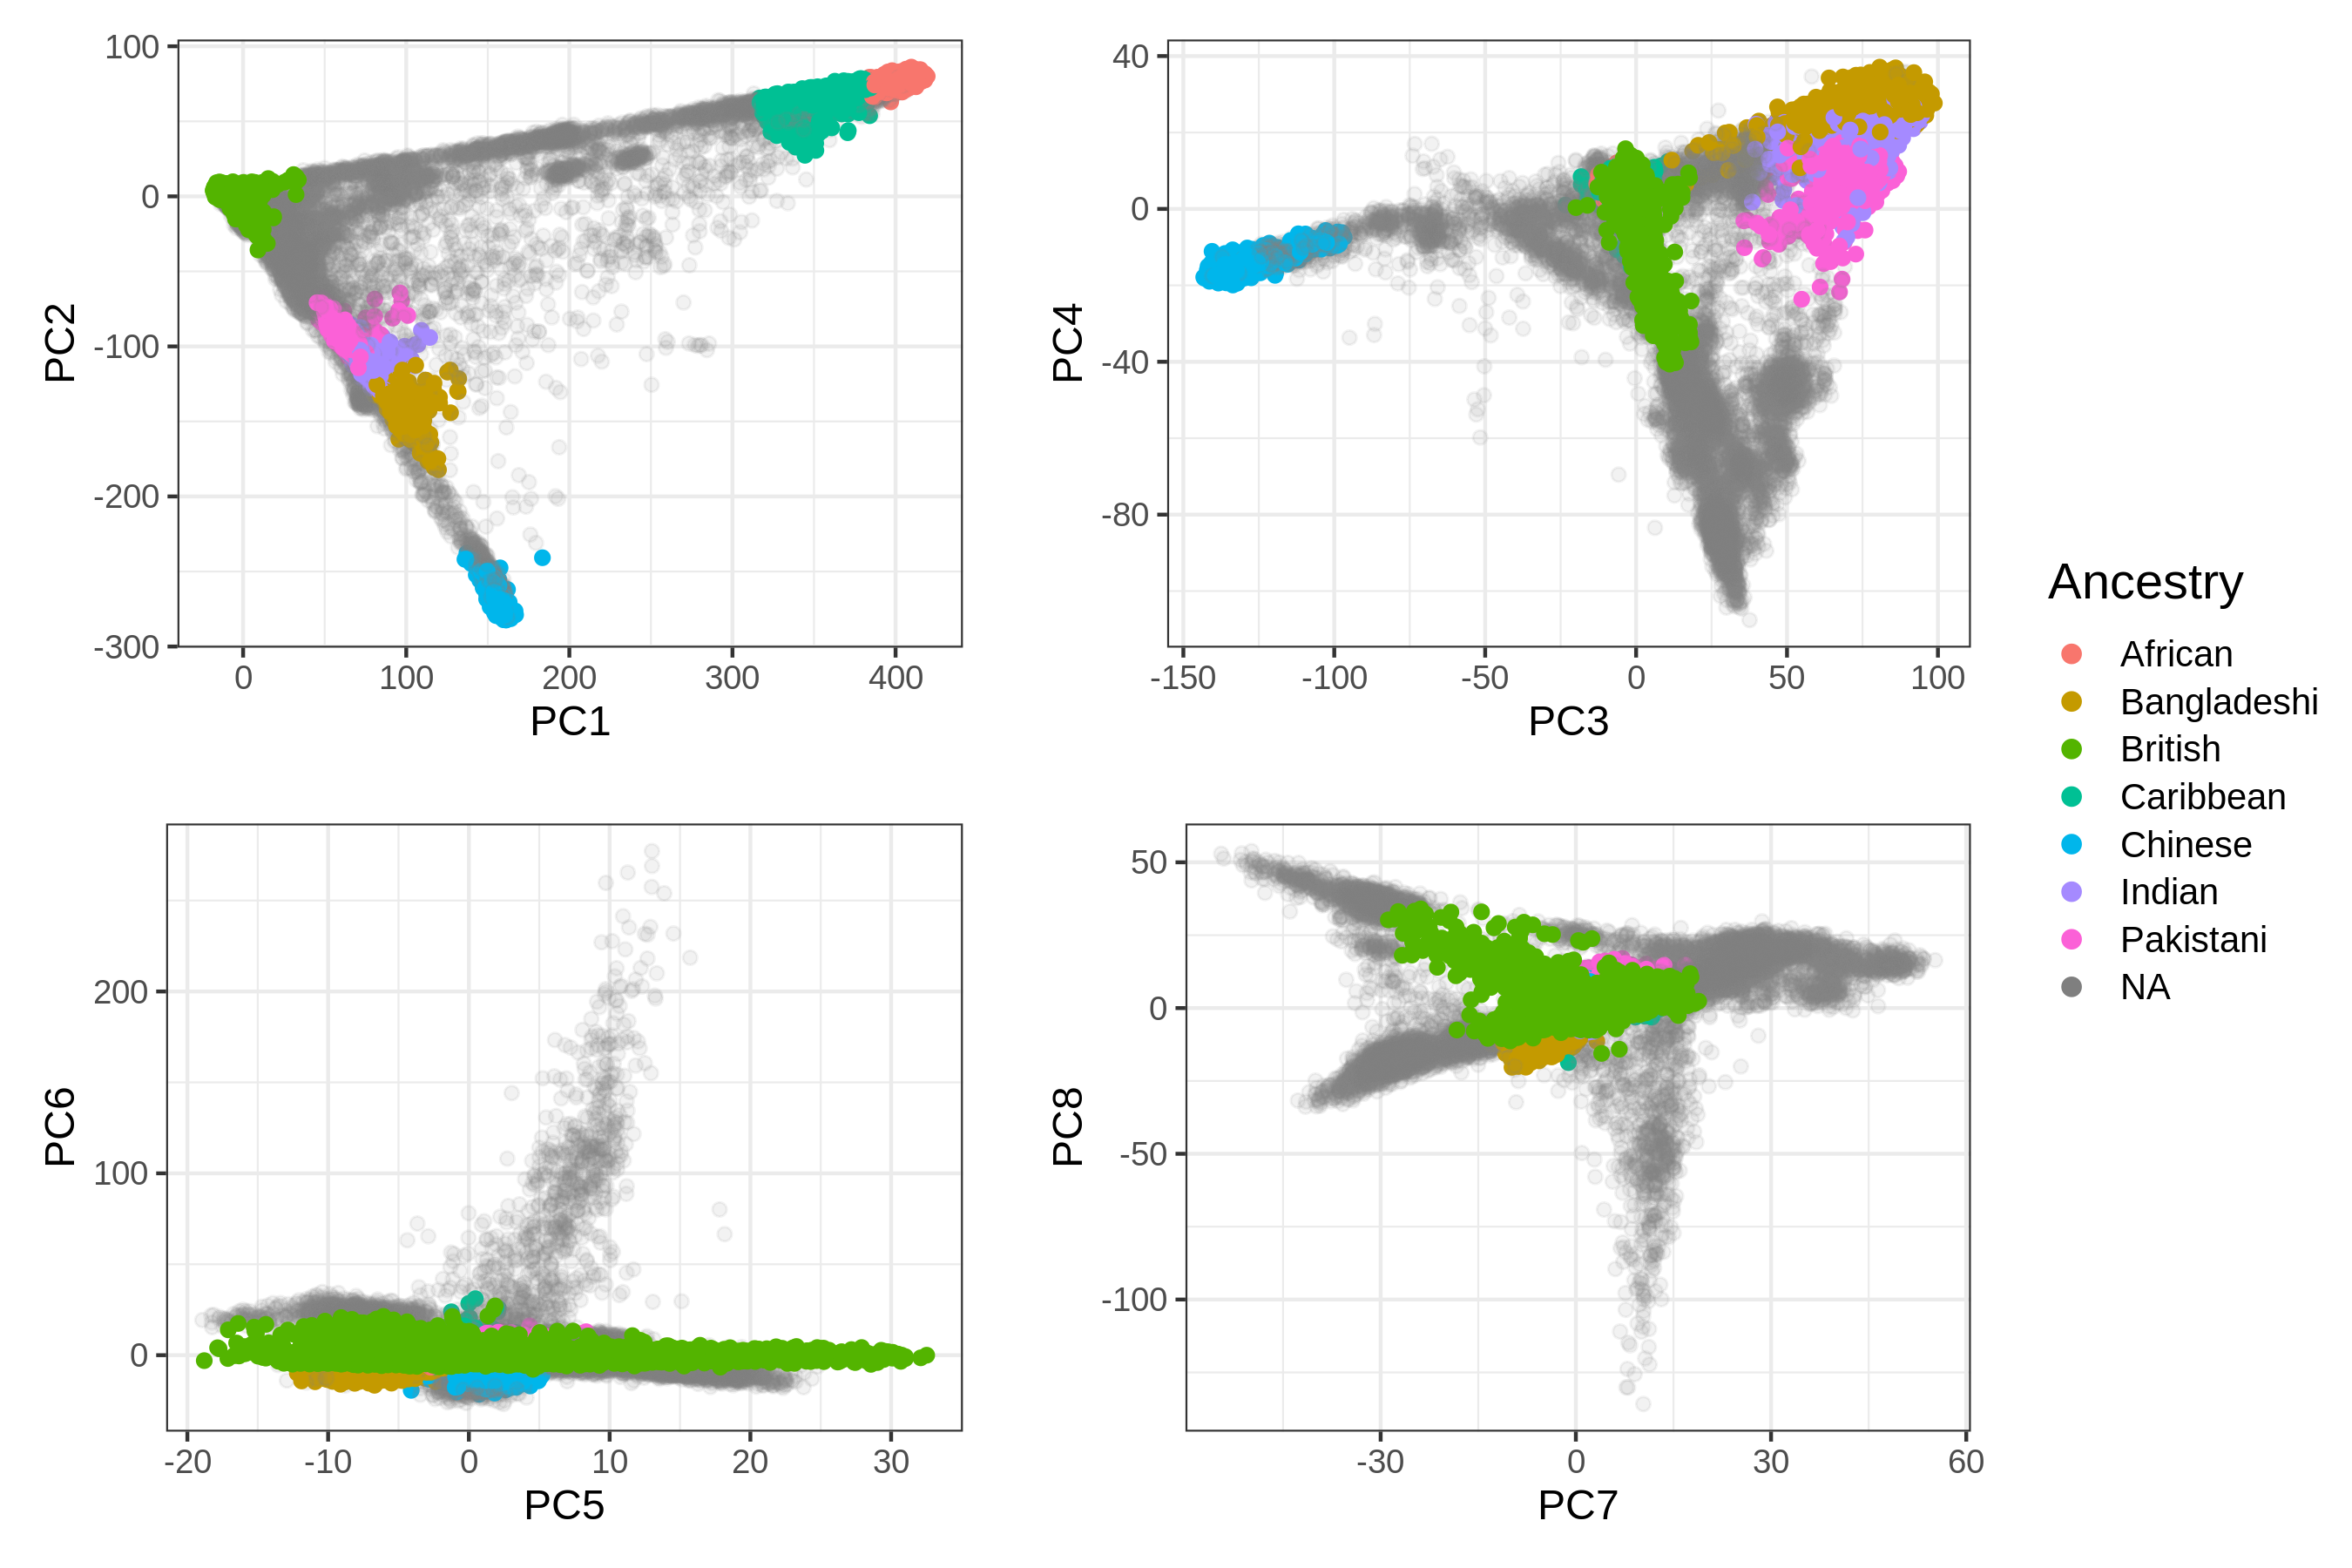
\includegraphics[width=0.95\textwidth]{UKBB-matched-ancestry}}
	\caption{ \label{fig:grouping}}
\end{figure}

%%%%%%%%%%%%%%%%%%%%%%%%%%%%%%%%%%%%%%%%%%%%%%%%%%%%%%%%%%%%%%%%%%%%%%%%%%%%%%%%

\subsection*{Discussion}

Here, we propose a PCA-based method for ancestry inference and grouping into genetically homogeneous clusters.
We show how the PCA-based distance is related to $F_{ST}$, which allows to compute distances based on PC scores directly.
Previously, we had proposed to use robust Mahalanobis distances to identify a homogeneous group of individuals \cite[]{prive2020efficient}. 
When looking at distances between two populations, this corresponds to using the Bhattacharyya distance, which appear suboptimal here compared to using a simple Euclidean distance.
We hypothesize that the main issue with this approach is that, when there is a very tight cluster, all distances to this cluster are large because of the covariance component in the Mahalanobis distance.
In contrast, here we propose to directly use the global scale of the PC scores, which is invariant from the cluster scattering.
This global scale makes it also more robust to infer ancestry with our method as compared to using relative proportions from k=20 nearest neighbors (kNN).
Indeed, consider an example of an admixed individual with say 25\% European ancestry and 75\% African ancestry.
The kNN-based method is likely to identify this individual as of African ancestry, while our method will probably be unable to match it, which is a beneficial feature when we are interested defining genetically homogeneous groups.

Yet, our proposed method has some limitations. 
First, since we match target individuals to 1000G populations, if individuals are far from all 26 1000G populations, then they would not be matched.
When looking at the POPRES data, more individuals from East Europe could not be matched. 
This is not surprising because there are no Eastern European population in the 1000G data.
Moreover, if we look at the location of the 1000G populations on a map (Figure \ref{fig:map}), we can see that it lacks representation of many parts of the world.
This issue has been reported e.g.\ for Asian populations \cite[]{lu2013principal}.
More diverse populations should be aggregated to better cover the worldwide genome diversity. This probably would make our method better and, if a sufficient coverage is achieved, we could approximate geographic coordinates by triangulation.
Then, we also show how to define homogeneous ancestry groups without the use of 1000G data.
When an predominant genetic ancestry is present in the data, such as British in the UK Biobank \cite[]{bycroft2017genome} or Danish in the iPSYCH data \cite[]{pedersen2018ipsych2012}, it is possible to directly rely on this to restrict to an homogeneous subset of the data.

A second potential limitation of our method is that it has two hyper-parameters: the number of PCs used to compute the distances and the threshold on the minimum distance to any cluster above which the ancestry is not matched. 
Many studies use only the first two PCs for ancestry inference. This is not enough to distinguish between Admixed Americans and South Asians (see AMR and SAS in figure \ref{fig:grouping}), let alone for distinguishing between populations at the sub-continental level.
As in \cite{prive2020efficient}, we recommend to use all PCs that visually separate some populations.
Moreover, we believe our method to be robust to the number of PCs used because contribution of later PCs is smaller than for first PCs.
For the distance limit, we have shown here how to define it to approximately correspond to an $F_{ST}$ of 0.002. Alternatively, a threshold can be chosen based on the visual inspection of the histogram of distances (on a log scale).
This threshold can also be adjusted depending on how stringent you want your selection to be.

In conclusion, we believe our proposed approach to be an easy way to infer global ancestry and to define groups of homogeneous ancestry.
This not a method to define admixture coefficients or infer local ancestry, which are different problems for which there are several existing methods \cite[]{alexander2009fast}.
However, inferring global ancestry in non-admixed individuals is still a very important problem since there are methods that specifically need to be applied in ancestry homogeneous samples.
This is the case e.g.\ for polygenic score methods that have been shown to underperform when applied to populations not homogeneous to the one used for training \cite[]{martin2017human}.

%%%%%%%%%%%%%%%%%%%%%%%%%%%%%%%%%%%%%%%%%%%%%%%%%%%%%%%%%%%%%%%%%%%%%%%%%%%%%%%%


\clearpage

\section*{Software and code availability}

The code used in this paper is available at \url{https://github.com/privefl/paper-ancestry-matching/tree/master/code}.

\section*{Acknowledgements}

\section*{Funding}

F.P.\ is supported by the Danish National Research Foundation (Niels Bohr Professorship to John McGrath).

\section*{Declaration of Interests}

The authors declare no competing interests.

%%%%%%%%%%%%%%%%%%%%%%%%%%%%%%%%%%%%%%%%%%%%%%%%%%%%%%%%%%%%%%%%%%%%%%%%%%%%%%%%

%\newpage

\bibliographystyle{natbib}
\bibliography{refs}

%%%%%%%%%%%%%%%%%%%%%%%%%%%%%%%%%%%%%%%%%%%%%%%%%%%%%%%%%%%%%%%%%%%%%%%%%%%%%%%%

\section*{Supplementary Materials}

\renewcommand{\thefigure}{S\arabic{figure}}
\setcounter{figure}{0}
\renewcommand{\thetable}{S\arabic{table}}
\setcounter{table}{0}
\renewcommand{\theequation}{S\arabic{equation}}
\setcounter{equation}{0}
\renewcommand{\thesection}{S\arabic{section}}
\setcounter{section}{1}

\subsection*{Definitions $\dag$ and methods}

[ALSO DESCRIBE 1000G DATA]

\begin{itemize}
	
	\item The $\boldsymbol{F_{ST}}$ measures the relative amount of genetic variance between populations compared to the total genetic variance within these populations \cite[]{wright1965interpretation}.
	We use the weighted average formula proposed in \cite{weir1984estimating}, which we now implement in our package bigsnpr \cite[]{prive2017efficient}.
	
	\item The {\bf Principal Component (PC) scores} are defined as $U \Delta$, where $U \Delta V^T$ is the singular value decomposition of the (scaled) genotype matrix. They are usually truncated, e.g.\ corresponding to the first 20 principal dimensions only. 
	
	\item The {\bf Bhattacharyya distance} between two multivariate normal distributions $\mathcal{N}(\boldsymbol\mu_1,\,\boldsymbol\Sigma_1)$ and $\mathcal{N}(\boldsymbol\mu_2,\,\boldsymbol\Sigma_2)$, which is defined as
	$D_B={1\over 8}(\boldsymbol\mu_2-\boldsymbol\mu_1)^T \boldsymbol\Sigma^{-1}(\boldsymbol\mu_2-\boldsymbol\mu_1)+{1\over 2}\log \,\left({|\boldsymbol\Sigma| \over \sqrt{|\boldsymbol\Sigma_1| \, |\boldsymbol\Sigma_2|} }\right)$,
	where $\boldsymbol\Sigma={\boldsymbol\Sigma_1+\boldsymbol\Sigma_2 \over 2}$ and $|M|$ is the absolute value of the determinant of matrix $M$ \cite[]{bhattacharyya1943measure,fukunaga1990introduction}. 
	The mean and covariance parameters for each population are computed using the robust location and covariance parameters as proposed in \cite{prive2020efficient}.
	
	\item The {\bf geometric median} of points is the point that minimizes the sum of all Euclidean distances to these points. We now implement this as function \texttt{geometric\_median} in our R package bigutilsr.
	
	\item The {\bf UK Biobank} is a large cohort of half a million individuals from the UK, for which we have access to both genotypes and multiple phenotypes (\url{https://www.ukbiobank.ac.uk/}).
	We apply some quality control filters to the genotyped data; we remove individuals with more than 10\% missing values, variants with more than 1\% missing values, variants having a minor allele frequency < 0.01, variants with P-value of the Hardy-Weinberg exact test < $10^{-50}$, and non-autosomal variants. 
	This results in 488,371 individuals and 504,139 genetic variants.
	
\end{itemize}

%%%%%%%%%%%%%%%%%%%%%%%%%%%%%%%%%%%%%%%%%%%%%%%%%%%%%%%%%%%%%%%%%%%%%%%%%%%%%%%%

\clearpage

\subsection*{Location of 1000G populations}

\begin{figure}[h]
	\centerline{\includegraphics[width=0.95\textwidth]{map-1000G}}
	\caption{ \label{fig:map}}
\end{figure}

%%%%%%%%%%%%%%%%%%%%%%%%%%%%%%%%%%%%%%%%%%%%%%%%%%%%%%%%%%%%%%%%%%%%%%%%%%%%%%%%

\clearpage

\subsection*{Measures of genetic dissimilarity between populations}

% latex table generated in R 3.6.1 by xtable 1.8-4 package
% Sun Sep 27 10:11:11 2020
\begin{table}[ht]
\centering
\caption{$F_{ST}$ values between African populations of the 1000G and all 26 1000G populations.} 
\label{tab:fst-AFR}
\begin{tabular}{|l|c|c|c|c|c|c|c|}
  \hline
 & LWK & ESN & YRI & ACB & ASW & GWD & MSL \\ 
  \hline
LWK & 0.0000 & 0.0077 & 0.0071 & 0.0064 & 0.0090 & 0.0108 & 0.0093 \\ 
  ESN & 0.0077 & 0.0000 & 0.0008 & 0.0034 & 0.0088 & 0.0075 & 0.0051 \\ 
  YRI & 0.0071 & 0.0008 & 0.0000 & 0.0025 & 0.0080 & 0.0062 & 0.0039 \\ 
  ACB & 0.0064 & 0.0034 & 0.0025 & 0.0000 & 0.0020 & 0.0060 & 0.0044 \\ 
  ASW & 0.0090 & 0.0088 & 0.0080 & 0.0020 & 0.0000 & 0.0098 & 0.0094 \\ 
  GWD & 0.0108 & 0.0075 & 0.0062 & 0.0060 & 0.0098 & 0.0000 & 0.0036 \\ 
  MSL & 0.0093 & 0.0051 & 0.0039 & 0.0044 & 0.0094 & 0.0036 & 0.0000 \\ 
   \hline
JPT & 0.1475 & 0.1564 & 0.1545 & 0.1344 & 0.1194 & 0.1517 & 0.1574 \\ 
  CHB & 0.1456 & 0.1546 & 0.1527 & 0.1324 & 0.1174 & 0.1499 & 0.1556 \\ 
  CHS & 0.1466 & 0.1555 & 0.1536 & 0.1335 & 0.1186 & 0.1509 & 0.1565 \\ 
  CDX & 0.1456 & 0.1544 & 0.1526 & 0.1324 & 0.1178 & 0.1498 & 0.1555 \\ 
  KHV & 0.1435 & 0.1525 & 0.1507 & 0.1304 & 0.1154 & 0.1479 & 0.1535 \\ 
   \hline
GIH & 0.1101 & 0.1200 & 0.1186 & 0.0954 & 0.0773 & 0.1156 & 0.1200 \\ 
  PJL & 0.1069 & 0.1167 & 0.1154 & 0.0920 & 0.0735 & 0.1124 & 0.1167 \\ 
  BEB & 0.1077 & 0.1174 & 0.1161 & 0.0934 & 0.0755 & 0.1131 & 0.1174 \\ 
  ITU & 0.1096 & 0.1195 & 0.1181 & 0.0954 & 0.0778 & 0.1151 & 0.1195 \\ 
  STU & 0.1091 & 0.1189 & 0.1175 & 0.0949 & 0.0774 & 0.1145 & 0.1189 \\ 
   \hline
PEL & 0.1472 & 0.1559 & 0.1541 & 0.1325 & 0.1144 & 0.1515 & 0.1567 \\ 
  MXL & 0.1125 & 0.1219 & 0.1205 & 0.0972 & 0.0772 & 0.1175 & 0.1218 \\ 
  CLM & 0.0970 & 0.1063 & 0.1051 & 0.0816 & 0.0620 & 0.1021 & 0.1061 \\ 
  PUR & 0.0849 & 0.0938 & 0.0927 & 0.0699 & 0.0515 & 0.0898 & 0.0935 \\ 
   \hline
FIN & 0.1219 & 0.1319 & 0.1306 & 0.1044 & 0.0837 & 0.1272 & 0.1319 \\ 
  CEU & 0.1189 & 0.1291 & 0.1278 & 0.1014 & 0.0805 & 0.1244 & 0.1290 \\ 
  GBR & 0.1193 & 0.1295 & 0.1282 & 0.1017 & 0.0808 & 0.1248 & 0.1294 \\ 
  IBS & 0.1145 & 0.1247 & 0.1234 & 0.0975 & 0.0772 & 0.1199 & 0.1247 \\ 
  TSI & 0.1154 & 0.1258 & 0.1245 & 0.0986 & 0.0783 & 0.1210 & 0.1258 \\ 
   \hline
\end{tabular}
\end{table}

% latex table generated in R 3.6.1 by xtable 1.8-4 package
% Sun Sep 27 10:11:11 2020
\begin{table}[ht]
\centering
\caption{$F_{ST}$ values between admixed American populations of the 1000G and all 26 1000G populations.} 
\label{tab:fst-AMR}
\begin{tabular}{|l|c|c|c|c|}
  \hline
 & PEL & MXL & CLM & PUR \\ 
  \hline
LWK & 0.1472 & 0.1125 & 0.0970 & 0.0849 \\ 
  ESN & 0.1559 & 0.1219 & 0.1063 & 0.0938 \\ 
  YRI & 0.1541 & 0.1205 & 0.1051 & 0.0927 \\ 
  ACB & 0.1325 & 0.0972 & 0.0816 & 0.0699 \\ 
  ASW & 0.1144 & 0.0772 & 0.0620 & 0.0515 \\ 
  GWD & 0.1515 & 0.1175 & 0.1021 & 0.0898 \\ 
  MSL & 0.1567 & 0.1218 & 0.1061 & 0.0935 \\ 
   \hline
JPT & 0.0795 & 0.0643 & 0.0707 & 0.0773 \\ 
  CHB & 0.0786 & 0.0628 & 0.0689 & 0.0752 \\ 
  CHS & 0.0811 & 0.0650 & 0.0708 & 0.0769 \\ 
  CDX & 0.0849 & 0.0675 & 0.0719 & 0.0773 \\ 
  KHV & 0.0817 & 0.0643 & 0.0689 & 0.0744 \\ 
   \hline
GIH & 0.0725 & 0.0370 & 0.0278 & 0.0269 \\ 
  PJL & 0.0688 & 0.0327 & 0.0230 & 0.0220 \\ 
  BEB & 0.0669 & 0.0344 & 0.0278 & 0.0282 \\ 
  ITU & 0.0732 & 0.0391 & 0.0308 & 0.0303 \\ 
  STU & 0.0728 & 0.0390 & 0.0309 & 0.0305 \\ 
   \hline
PEL & 0.0000 & 0.0170 & 0.0380 & 0.0548 \\ 
  MXL & 0.0170 & 0.0000 & 0.0090 & 0.0180 \\ 
  CLM & 0.0380 & 0.0090 & 0.0000 & 0.0056 \\ 
  PUR & 0.0548 & 0.0180 & 0.0056 & 0.0000 \\ 
   \hline
FIN & 0.0772 & 0.0338 & 0.0178 & 0.0149 \\ 
  CEU & 0.0804 & 0.0334 & 0.0143 & 0.0100 \\ 
  GBR & 0.0809 & 0.0338 & 0.0146 & 0.0102 \\ 
  IBS & 0.0820 & 0.0339 & 0.0134 & 0.0081 \\ 
  TSI & 0.0825 & 0.0345 & 0.0143 & 0.0090 \\ 
   \hline
\end{tabular}
\end{table}

% latex table generated in R 3.6.1 by xtable 1.8-4 package
% Sun Sep 27 10:11:11 2020
\begin{table}[ht]
\centering
\caption{$F_{ST}$ values between East Asian populations of the 1000G and all 26 1000G populations.} 
\label{tab:fst-EAS}
\begin{tabular}{|l|c|c|c|c|c|}
  \hline
 & JPT & CHB & CHS & CDX & KHV \\ 
  \hline
LWK & 0.1475 & 0.1456 & 0.1466 & 0.1456 & 0.1435 \\ 
  ESN & 0.1564 & 0.1546 & 0.1555 & 0.1544 & 0.1525 \\ 
  YRI & 0.1545 & 0.1527 & 0.1536 & 0.1526 & 0.1507 \\ 
  ACB & 0.1344 & 0.1324 & 0.1335 & 0.1324 & 0.1304 \\ 
  ASW & 0.1194 & 0.1174 & 0.1186 & 0.1178 & 0.1154 \\ 
  GWD & 0.1517 & 0.1499 & 0.1509 & 0.1498 & 0.1479 \\ 
  MSL & 0.1574 & 0.1556 & 0.1565 & 0.1555 & 0.1535 \\ 
   \hline
JPT & 0.0000 & 0.0068 & 0.0086 & 0.0166 & 0.0140 \\ 
  CHB & 0.0068 & 0.0000 & 0.0010 & 0.0084 & 0.0062 \\ 
  CHS & 0.0086 & 0.0010 & 0.0000 & 0.0047 & 0.0031 \\ 
  CDX & 0.0166 & 0.0084 & 0.0047 & 0.0000 & 0.0016 \\ 
  KHV & 0.0140 & 0.0062 & 0.0031 & 0.0016 & 0.0000 \\ 
   \hline
GIH & 0.0693 & 0.0673 & 0.0685 & 0.0685 & 0.0650 \\ 
  PJL & 0.0669 & 0.0647 & 0.0660 & 0.0660 & 0.0626 \\ 
  BEB & 0.0542 & 0.0518 & 0.0528 & 0.0527 & 0.0494 \\ 
  ITU & 0.0656 & 0.0636 & 0.0647 & 0.0646 & 0.0611 \\ 
  STU & 0.0642 & 0.0623 & 0.0634 & 0.0633 & 0.0598 \\ 
   \hline
PEL & 0.0795 & 0.0786 & 0.0811 & 0.0849 & 0.0817 \\ 
  MXL & 0.0643 & 0.0628 & 0.0650 & 0.0675 & 0.0643 \\ 
  CLM & 0.0707 & 0.0689 & 0.0708 & 0.0719 & 0.0689 \\ 
  PUR & 0.0773 & 0.0752 & 0.0769 & 0.0773 & 0.0744 \\ 
   \hline
FIN & 0.0924 & 0.0901 & 0.0920 & 0.0925 & 0.0893 \\ 
  CEU & 0.0985 & 0.0960 & 0.0977 & 0.0978 & 0.0946 \\ 
  GBR & 0.0993 & 0.0968 & 0.0985 & 0.0985 & 0.0953 \\ 
  IBS & 0.0981 & 0.0957 & 0.0973 & 0.0973 & 0.0942 \\ 
  TSI & 0.0981 & 0.0956 & 0.0972 & 0.0972 & 0.0940 \\ 
   \hline
\end{tabular}
\end{table}

% latex table generated in R 3.6.1 by xtable 1.8-4 package
% Sun Sep 27 10:11:11 2020
\begin{table}[ht]
\centering
\caption{$F_{ST}$ values between European populations of the 1000G and all 26 1000G populations.} 
\label{tab:fst-EUR}
\begin{tabular}{|l|c|c|c|c|c|}
  \hline
 & FIN & CEU & GBR & IBS & TSI \\ 
  \hline
LWK & 0.1219 & 0.1189 & 0.1193 & 0.1145 & 0.1154 \\ 
  ESN & 0.1319 & 0.1291 & 0.1295 & 0.1247 & 0.1258 \\ 
  YRI & 0.1306 & 0.1278 & 0.1282 & 0.1234 & 0.1245 \\ 
  ACB & 0.1044 & 0.1014 & 0.1017 & 0.0975 & 0.0986 \\ 
  ASW & 0.0837 & 0.0805 & 0.0808 & 0.0772 & 0.0783 \\ 
  GWD & 0.1272 & 0.1244 & 0.1248 & 0.1199 & 0.1210 \\ 
  MSL & 0.1319 & 0.1290 & 0.1294 & 0.1247 & 0.1258 \\ 
   \hline
JPT & 0.0924 & 0.0985 & 0.0993 & 0.0981 & 0.0981 \\ 
  CHB & 0.0901 & 0.0960 & 0.0968 & 0.0957 & 0.0956 \\ 
  CHS & 0.0920 & 0.0977 & 0.0985 & 0.0973 & 0.0972 \\ 
  CDX & 0.0925 & 0.0978 & 0.0985 & 0.0973 & 0.0972 \\ 
  KHV & 0.0893 & 0.0946 & 0.0953 & 0.0942 & 0.0940 \\ 
   \hline
GIH & 0.0343 & 0.0325 & 0.0328 & 0.0334 & 0.0317 \\ 
  PJL & 0.0289 & 0.0269 & 0.0272 & 0.0278 & 0.0262 \\ 
  BEB & 0.0372 & 0.0368 & 0.0372 & 0.0375 & 0.0362 \\ 
  ITU & 0.0393 & 0.0380 & 0.0384 & 0.0384 & 0.0367 \\ 
  STU & 0.0398 & 0.0385 & 0.0389 & 0.0389 & 0.0373 \\ 
   \hline
PEL & 0.0772 & 0.0804 & 0.0809 & 0.0820 & 0.0825 \\ 
  MXL & 0.0338 & 0.0334 & 0.0338 & 0.0339 & 0.0345 \\ 
  CLM & 0.0178 & 0.0143 & 0.0146 & 0.0134 & 0.0143 \\ 
  PUR & 0.0149 & 0.0100 & 0.0102 & 0.0081 & 0.0090 \\ 
   \hline
FIN & 0.0000 & 0.0062 & 0.0066 & 0.0101 & 0.0116 \\ 
  CEU & 0.0062 & 0.0000 & 0.0002 & 0.0022 & 0.0034 \\ 
  GBR & 0.0066 & 0.0002 & 0.0000 & 0.0024 & 0.0037 \\ 
  IBS & 0.0101 & 0.0022 & 0.0024 & 0.0000 & 0.0015 \\ 
  TSI & 0.0116 & 0.0034 & 0.0037 & 0.0015 & 0.0000 \\ 
   \hline
\end{tabular}
\end{table}

% latex table generated in R 3.6.1 by xtable 1.8-4 package
% Sun Sep 27 10:11:11 2020
\begin{table}[ht]
\centering
\caption{$F_{ST}$ values between South Asian populations of the 1000G and all 26 1000G populations.} 
\label{tab:fst-SAS}
\begin{tabular}{|l|c|c|c|c|c|}
  \hline
 & GIH & PJL & BEB & ITU & STU \\ 
  \hline
LWK & 0.1101 & 0.1069 & 0.1077 & 0.1096 & 0.1091 \\ 
  ESN & 0.1200 & 0.1167 & 0.1174 & 0.1195 & 0.1189 \\ 
  YRI & 0.1186 & 0.1154 & 0.1161 & 0.1181 & 0.1175 \\ 
  ACB & 0.0954 & 0.0920 & 0.0934 & 0.0954 & 0.0949 \\ 
  ASW & 0.0773 & 0.0735 & 0.0755 & 0.0778 & 0.0774 \\ 
  GWD & 0.1156 & 0.1124 & 0.1131 & 0.1151 & 0.1145 \\ 
  MSL & 0.1200 & 0.1167 & 0.1174 & 0.1195 & 0.1189 \\ 
   \hline
JPT & 0.0693 & 0.0669 & 0.0542 & 0.0656 & 0.0642 \\ 
  CHB & 0.0673 & 0.0647 & 0.0518 & 0.0636 & 0.0623 \\ 
  CHS & 0.0685 & 0.0660 & 0.0528 & 0.0647 & 0.0634 \\ 
  CDX & 0.0685 & 0.0660 & 0.0527 & 0.0646 & 0.0633 \\ 
  KHV & 0.0650 & 0.0626 & 0.0494 & 0.0611 & 0.0598 \\ 
   \hline
GIH & 0.0000 & 0.0035 & 0.0042 & 0.0039 & 0.0043 \\ 
  PJL & 0.0035 & 0.0000 & 0.0035 & 0.0033 & 0.0036 \\ 
  BEB & 0.0042 & 0.0035 & 0.0000 & 0.0022 & 0.0021 \\ 
  ITU & 0.0039 & 0.0033 & 0.0022 & 0.0000 & 0.0013 \\ 
  STU & 0.0043 & 0.0036 & 0.0021 & 0.0013 & 0.0000 \\ 
   \hline
PEL & 0.0725 & 0.0688 & 0.0669 & 0.0732 & 0.0728 \\ 
  MXL & 0.0370 & 0.0327 & 0.0344 & 0.0391 & 0.0390 \\ 
  CLM & 0.0278 & 0.0230 & 0.0278 & 0.0308 & 0.0309 \\ 
  PUR & 0.0269 & 0.0220 & 0.0282 & 0.0303 & 0.0305 \\ 
   \hline
FIN & 0.0343 & 0.0289 & 0.0372 & 0.0393 & 0.0398 \\ 
  CEU & 0.0325 & 0.0269 & 0.0368 & 0.0380 & 0.0385 \\ 
  GBR & 0.0328 & 0.0272 & 0.0372 & 0.0384 & 0.0389 \\ 
  IBS & 0.0334 & 0.0278 & 0.0375 & 0.0384 & 0.0389 \\ 
  TSI & 0.0317 & 0.0262 & 0.0362 & 0.0367 & 0.0373 \\ 
   \hline
\end{tabular}
\end{table}


\begin{figure}[h]
	\centerline{\includegraphics[width=0.8\textwidth]{compare-dist-to-Fst}}
	\caption{Comparing Fst to different distances in the PCA space between pairs of the 26 1000G populations. \label{fig:compare-dist}}
\end{figure}

\begin{figure}[h]
\centerline{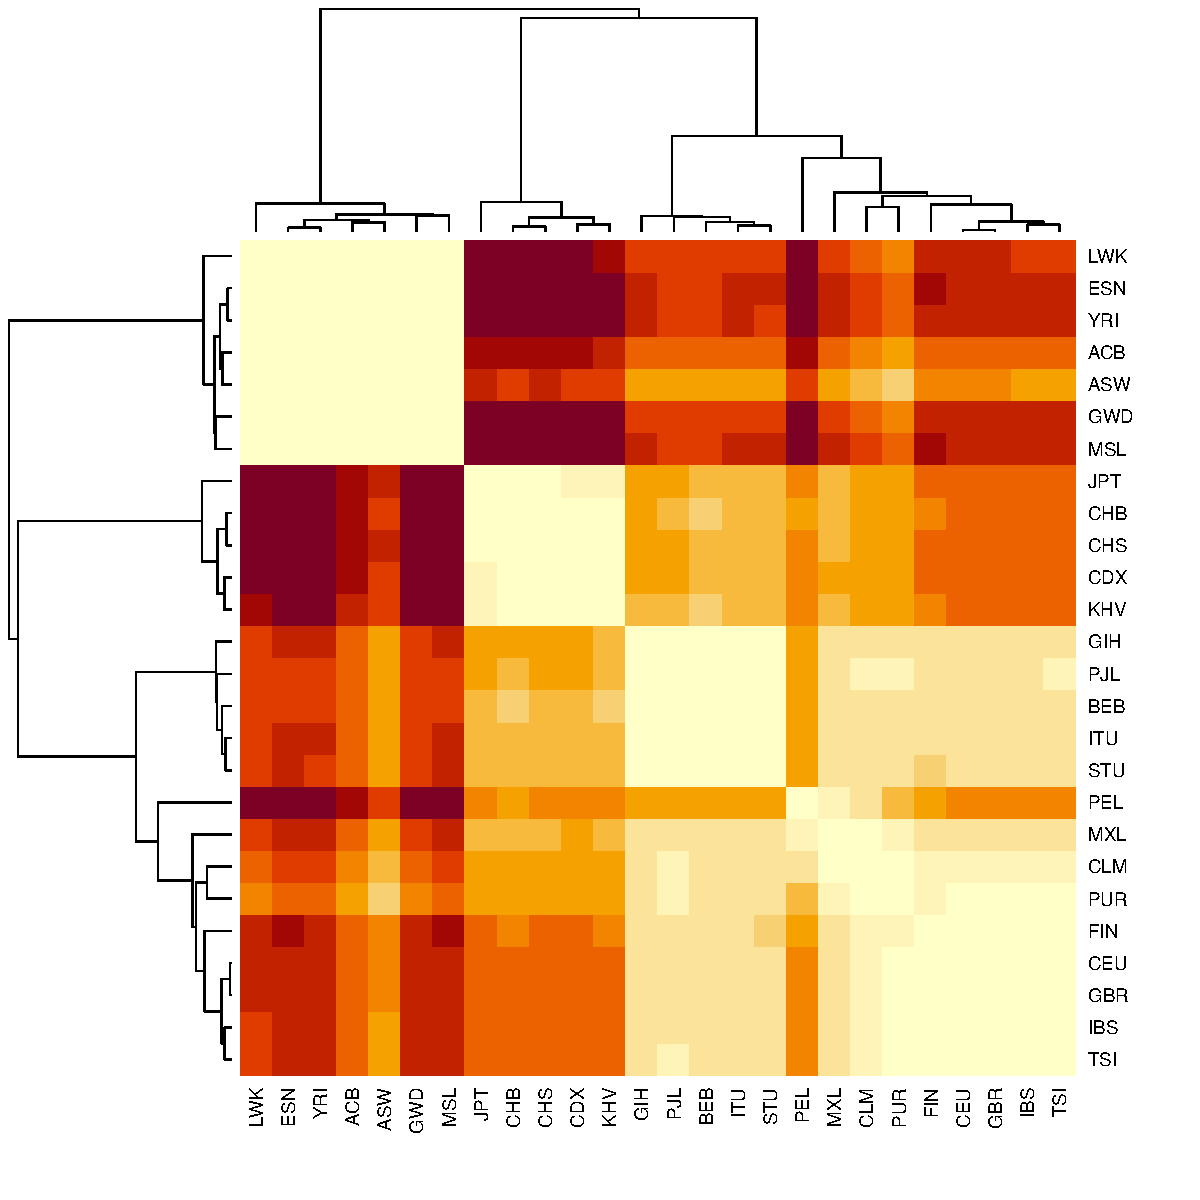
\includegraphics[width=0.8\textwidth]{heatmap-Fst-1000G}}
\caption{Heatmap with clustering based on the $F_{ST}$ between pairs of the 26 1000G populations. Corresponding values are reported in table S1-S5. \label{fig:heatmap0}}
\end{figure}

\begin{figure}[h]
	\centerline{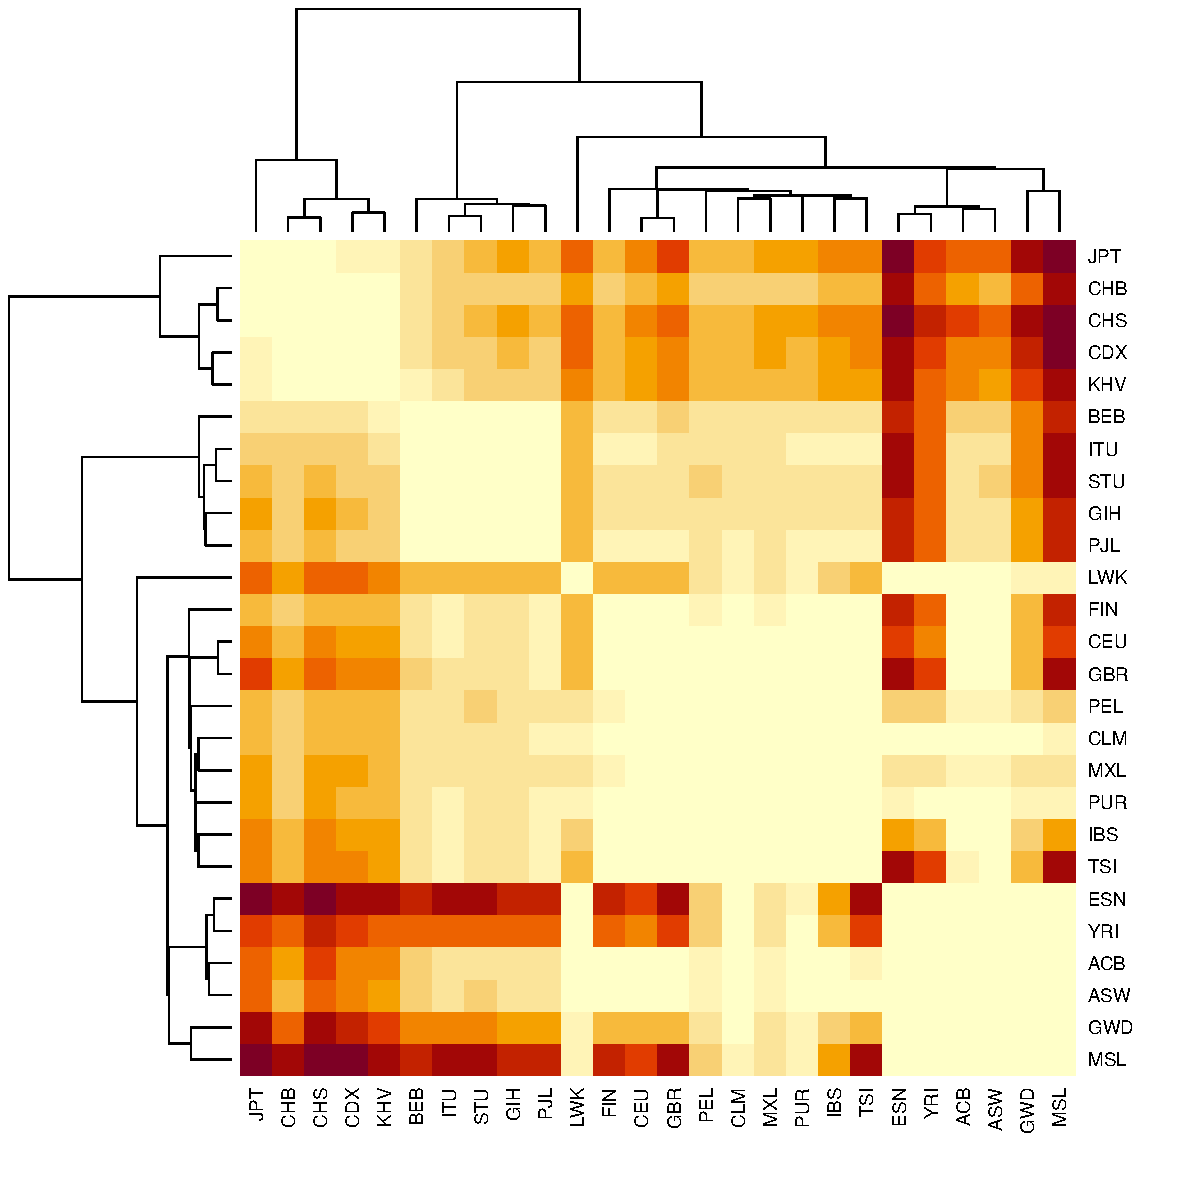
\includegraphics[width=0.8\textwidth]{heatmap-bhattacharyya-1000G}}
	\caption{Heatmap with clustering based on the Bhattacharyya distances between pairs of the 26 1000G populations. \label{fig:heatmap1}}
\end{figure}

\begin{figure}[h]
	\centerline{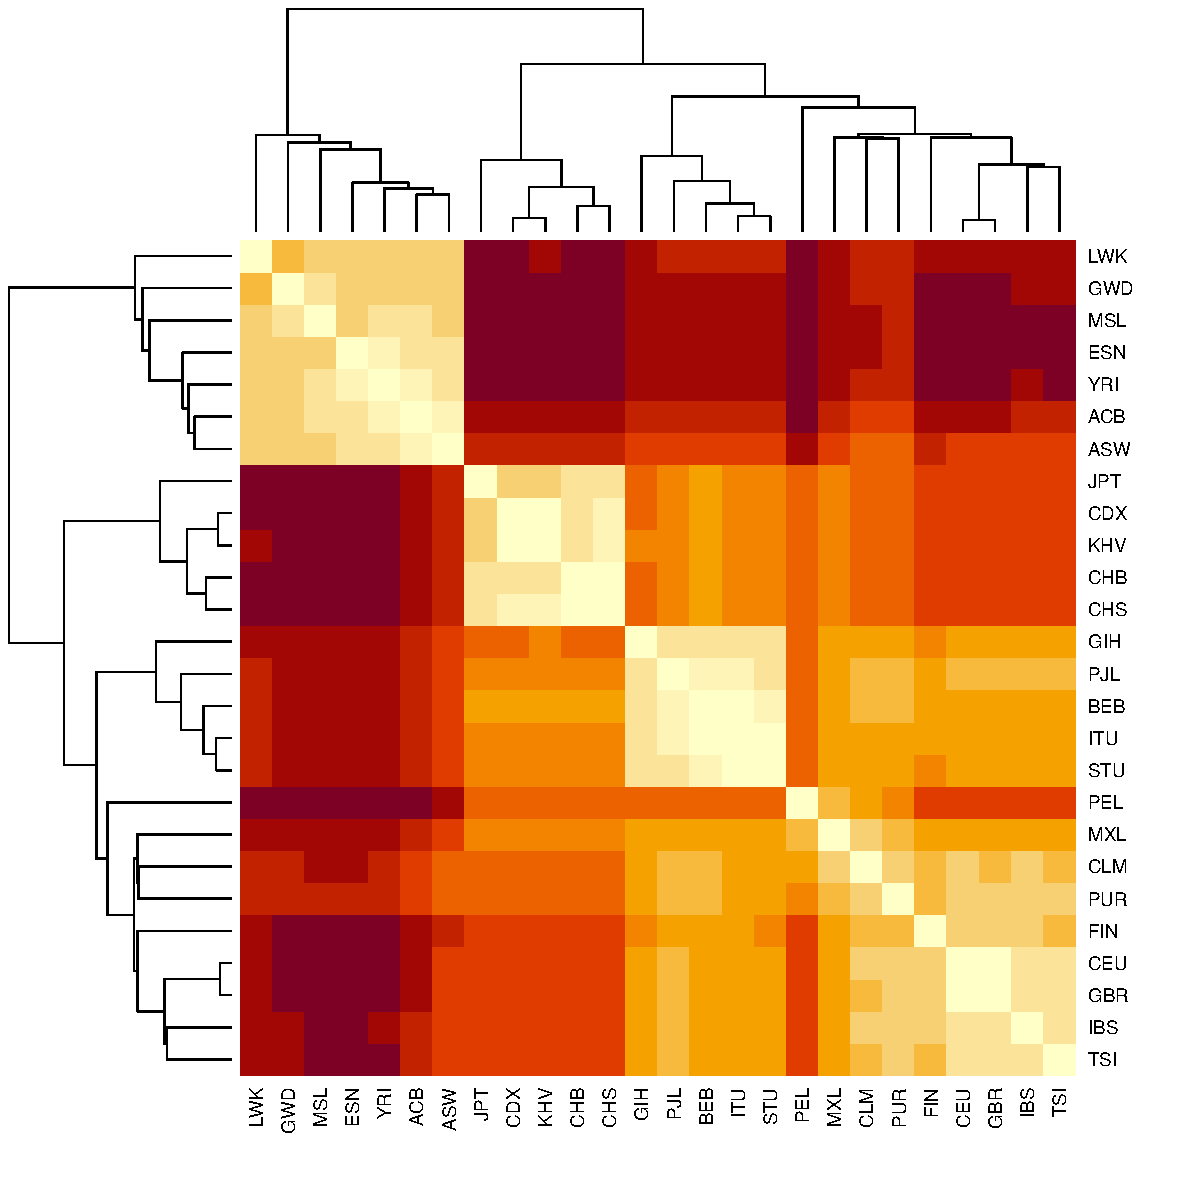
\includegraphics[width=0.8\textwidth]{heatmap-centers-1000G}}
	\caption{Heatmap with clustering based on the distances between centers of pairs of the 26 1000G populations. \label{fig:heatmap2}}
\end{figure}

\begin{figure}[h]
	\centerline{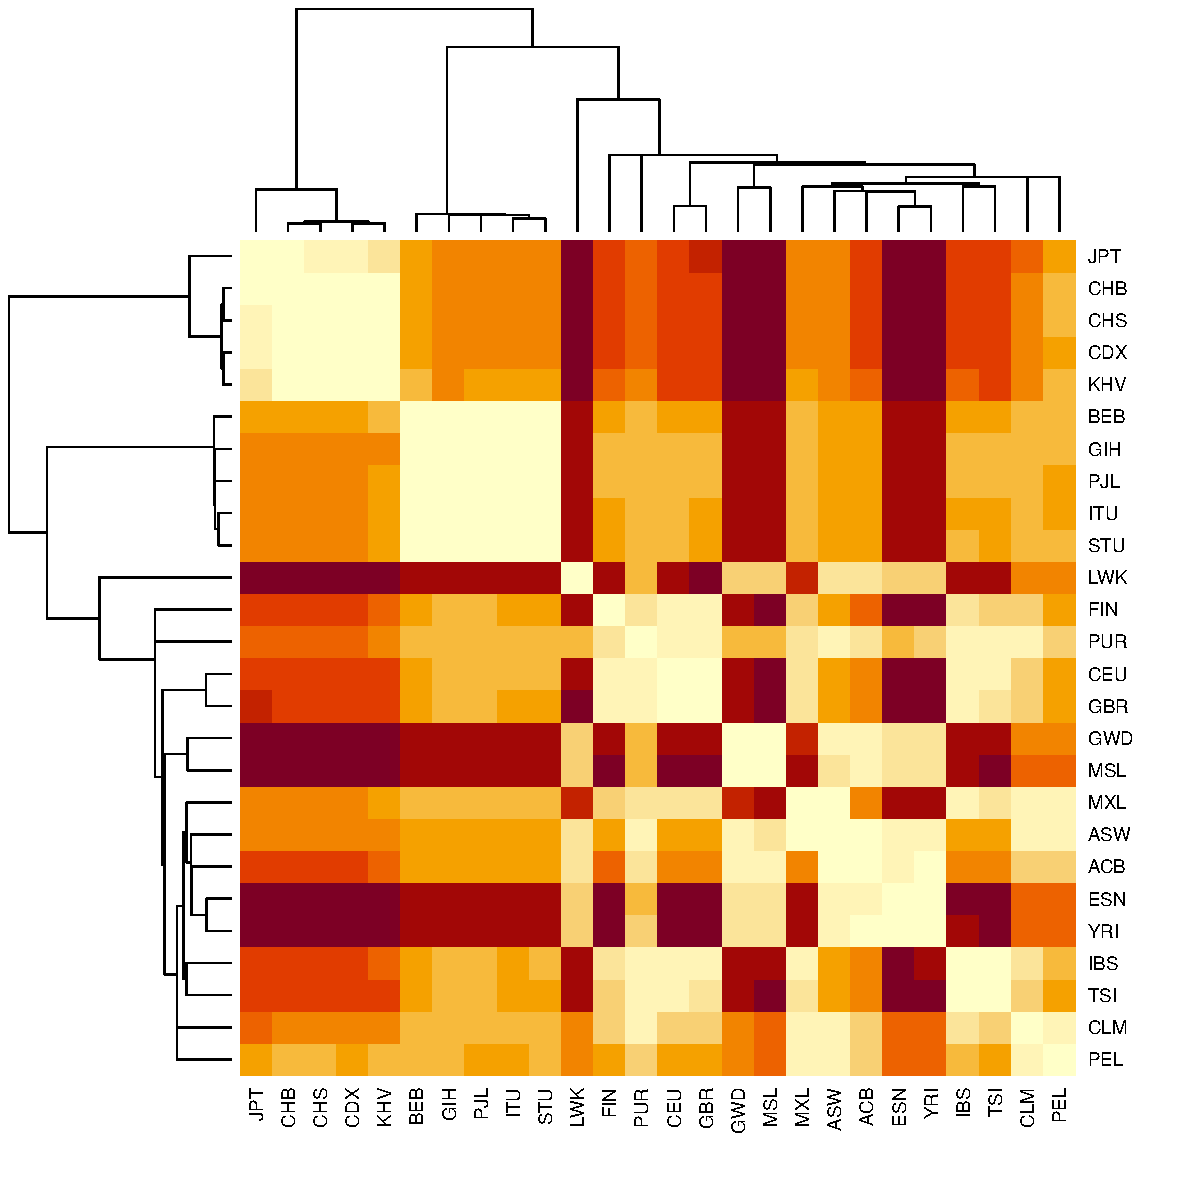
\includegraphics[width=0.8\textwidth]{heatmap-closest-1000G}}
	\caption{Heatmap with clustering based on the shortest distances between pairs of the 26 1000G populations. \label{fig:heatmap3}}
\end{figure}

\FloatBarrier

%%%%%%%%%%%%%%%%%%%%%%%%%%%%%%%%%%%%%%%%%%%%%%%%%%%%%%%%%%%%%%%%%%%%%%%%%%%%%%%%

\subsection*{PCA-based ancestry inference}

\begin{figure}[h]
	\centerline{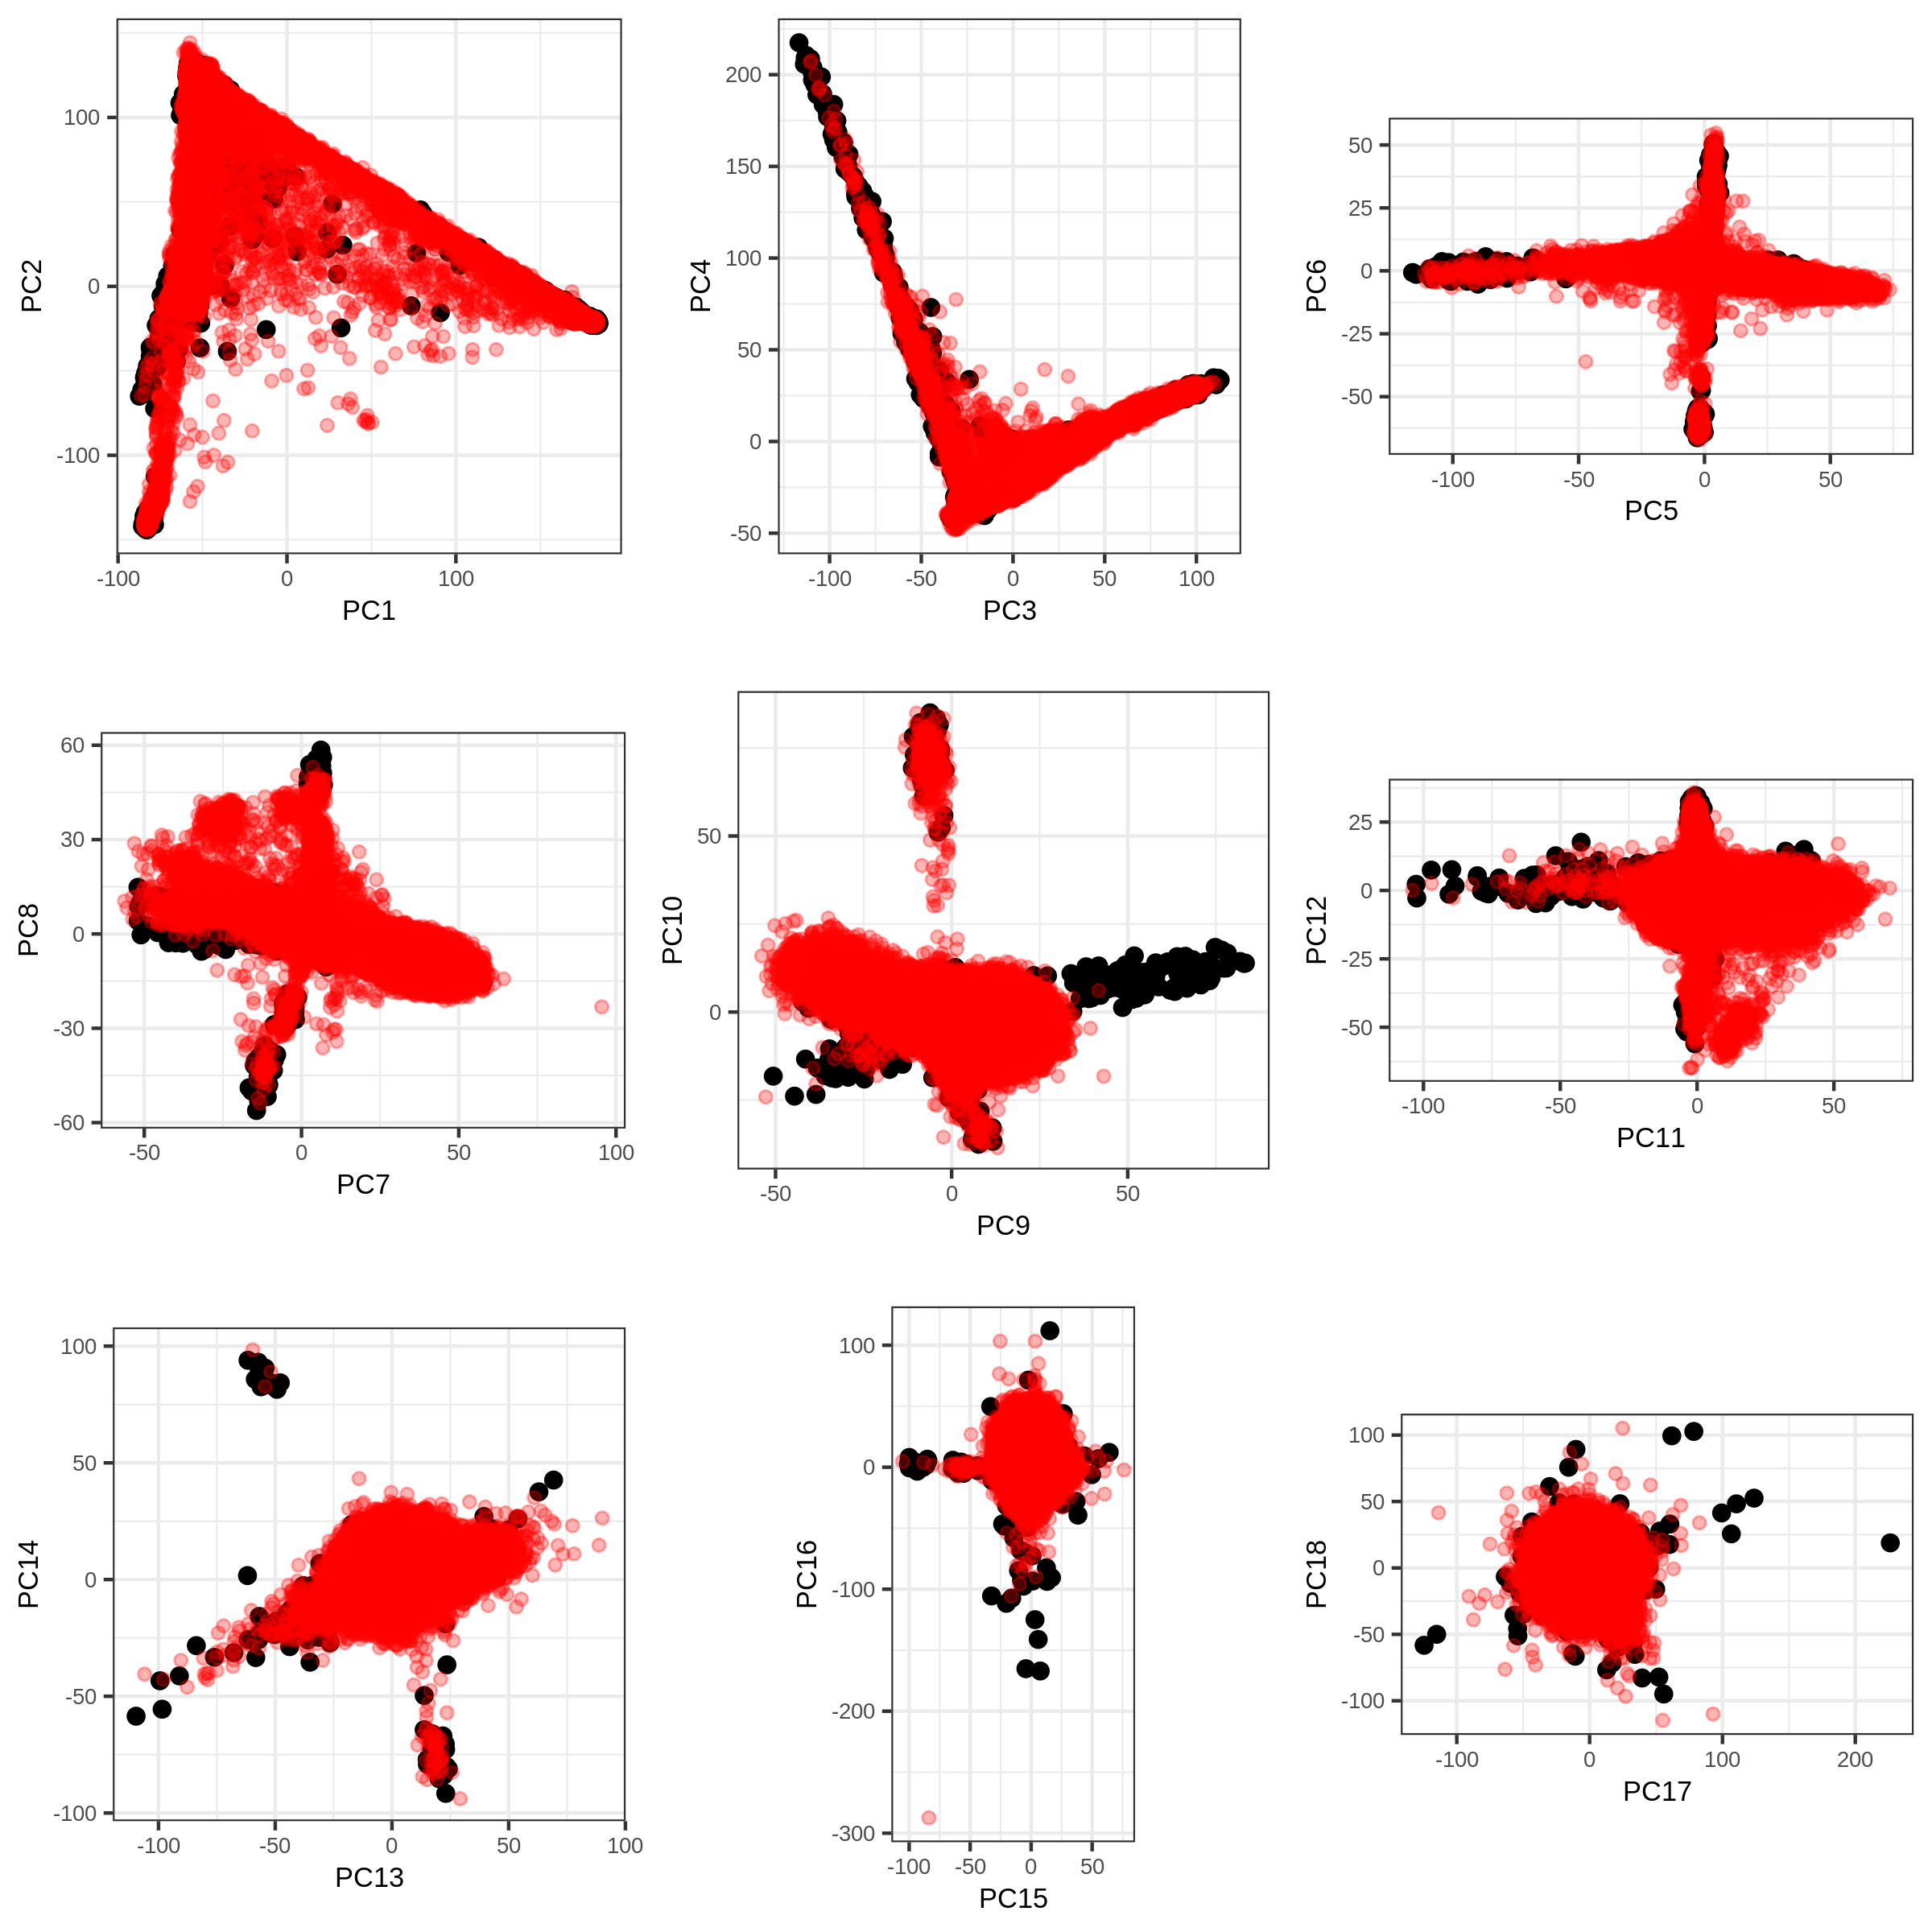
\includegraphics[width=0.95\textwidth]{proj-UKBB-to-1000G}}
	\caption{First 18 PC scores of the 1000G data (in black), onto which the UK Biobank data has been projected (in red). \label{fig:proj-UKBB}}
\end{figure}

\begin{figure}[h]
	\centerline{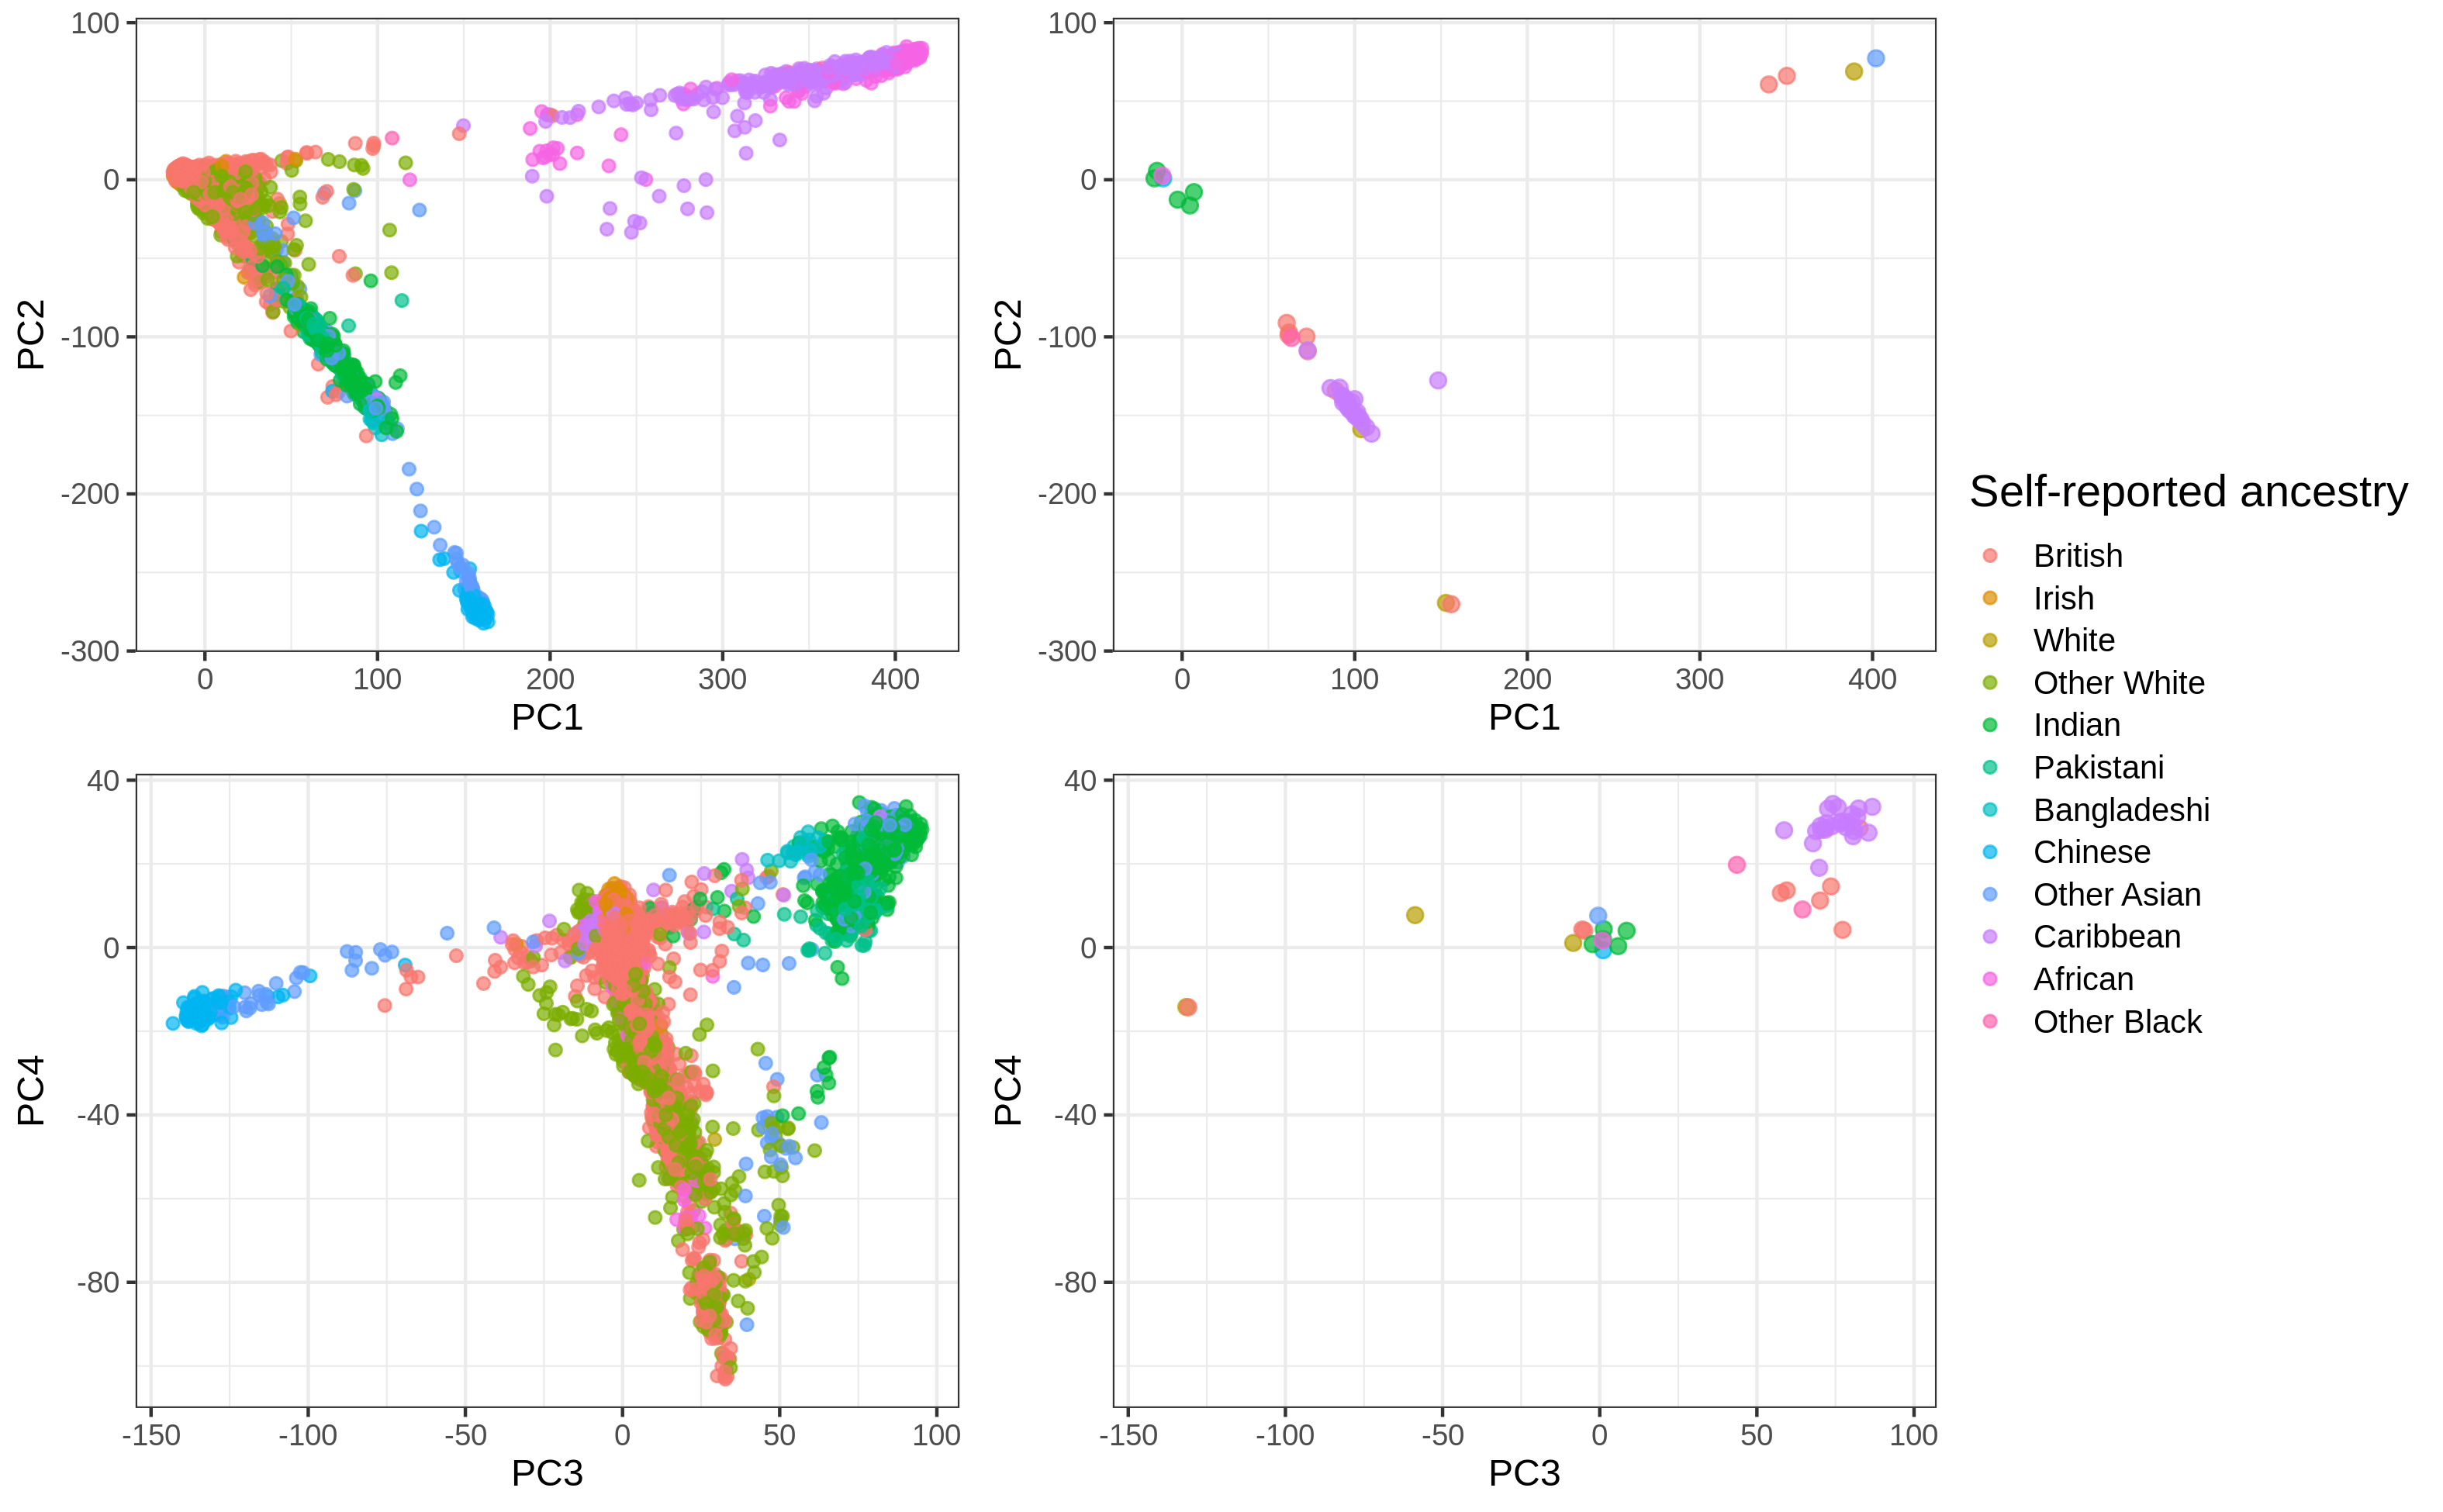
\includegraphics[width=0.95\textwidth]{UKBB-mismatch}}
	\caption{PC scores (computed in the UK Biobank) colored by self-reported ancestry. On the left, these are 50,000 random individuals. On the right, these are the 47 individuals with some discrepancy between their self-reported-ancestry and or ancestry estimation. \label{fig:mismatch}}
\end{figure}

% latex table generated in R 3.6.1 by xtable 1.8-4 package
% Sun Sep 27 14:34:15 2020
\begin{table}[ht]
\centering
\caption{Self-reported ancestry (left) of UKBB individuals and their matching to 1000G continental populations (top) using 20-wNN. See the description of 1000G populations at \url{https://www.internationalgenome.org/category/population/}.} 
\label{tab:ancestry-pred-kNN}
\begin{tabular}{|l|c|c|c|c|c|c|}
  \hline
 & AFR & AMR & EAS & EUR & SAS & Not matched \\ 
  \hline
British & 4 & 50 & 6 & 430696 & 95 & 163 \\ 
  Irish &  &  &  & 12748 & 3 & 2 \\ 
  White & 1 & 2 & 1 & 540 & 1 &  \\ 
  Other White &  & 170 & 1 & 15533 & 18 & 93 \\ 
   \hline
Indian &  &  &  & 21 & 5680 & 15 \\ 
  Pakistani &  &  &  & 3 & 1742 & 3 \\ 
  Bangladeshi &  &  &  &  & 220 & 1 \\ 
  Chinese &  & 7 & 1483 & 3 & 3 & 8 \\ 
  Other Asian & 1 & 1 & 359 & 216 & 1138 & 32 \\ 
   \hline
Caribbean & 4117 & 1 &  &  & 36 & 143 \\ 
  African & 3000 &  & 1 & 2 & 2 & 199 \\ 
  Other Black & 90 & 1 &  & 1 & 5 & 21 \\ 
   \hline
Asian or Asian British &  &  & 2 & 4 & 34 & 2 \\ 
  Black or Black British & 23 &  &  & 2 &  & 1 \\ 
  White and Black Caribbean & 93 & 16 &  & 74 & 11 & 403 \\ 
  White and Black African & 102 & 13 &  & 52 & 4 & 231 \\ 
  White and Asian &  & 42 & 10 & 242 & 349 & 159 \\ 
   \hline
Unknown  & 1024 & 541 & 712 & 3774 & 1020 & 749 \\ 
   \hline
\end{tabular}
\end{table}

% latex table generated in R 3.6.1 by xtable 1.8-4 package
% Sun Sep 27 14:29:28 2020
\begin{table}[ht]
\centering
\caption{Self-reported ancestry (top) of UKBB individuals and their matching to 1000G populations (left) by our method. See the description of 1000G populations at \url{https://www.internationalgenome.org/category/population/}.} 
\label{tab:ancestry-fine-pred}
\begin{tabular}{|l|c|c|c|c|c|c|c|c|c|c|c|c|c|}
  \hline
 & British & Irish & White & Other White & Indian & Pakistani & Bangladeshi & Chinese & Other Asian & Caribbean & African & Other Black & Unknown \\ 
  \hline
AFR\_ACB &  &  &  &  &  &  &  &  &  & 2024 & 66 & 34 & 198 \\ 
  AFR\_ASW & 2 &  &  &  &  &  &  &  &  & 1072 & 31 & 11 & 134 \\ 
  AFR\_ESN &  &  &  &  &  &  &  &  &  & 1 & 270 & 1 & 47 \\ 
  AFR\_GWD &  &  &  &  &  &  &  &  &  &  & 42 &  & 9 \\ 
  AFR\_LWK &  &  & 1 &  &  &  &  &  &  &  & 284 & 1 & 69 \\ 
  AFR\_MSL &  &  &  &  &  &  &  &  &  & 3 & 144 & 3 & 23 \\ 
  AFR\_YRI &  &  &  &  &  &  &  &  & 1 & 748 & 1796 & 24 & 404 \\ 
   \hline
AMR\_CLM &  &  &  & 18 &  &  &  &  &  &  &  &  & 27 \\ 
  AMR\_MXL &  &  &  & 21 &  &  &  &  &  &  &  &  & 117 \\ 
  AMR\_PEL &  &  & 1 & 1 &  &  &  &  &  &  &  &  & 30 \\ 
  AMR\_PUR &  &  &  &  &  &  &  &  &  &  &  &  & 1 \\ 
   \hline
EAS\_CDX &  &  &  &  &  &  &  & 4 & 15 &  &  &  & 10 \\ 
  EAS\_CHB &  &  &  &  &  &  &  & 218 & 23 &  &  &  & 33 \\ 
  EAS\_CHS & 1 &  & 1 &  &  &  &  & 907 & 17 &  &  &  & 42 \\ 
  EAS\_JPT &  &  &  &  &  &  &  & 10 & 53 &  &  &  & 221 \\ 
  EAS\_KHV &  &  &  &  &  &  &  & 314 & 171 &  &  &  & 274 \\ 
   \hline
EUR\_CEU & 183646 & 854 & 181 & 5802 & 2 &  &  & 1 &  &  &  &  & 883 \\ 
  EUR\_FIN & 1 &  &  & 126 &  &  &  &  &  &  &  &  & 1 \\ 
  EUR\_GBR & 235579 & 11461 & 294 & 2446 & 3 &  &  &  &  &  & 1 &  & 1066 \\ 
  EUR\_IBS & 68 &  & 7 & 775 &  &  &  &  &  &  &  &  & 24 \\ 
  EUR\_TSI & 2163 & 13 & 17 & 2185 &  &  &  &  &  &  &  &  & 365 \\ 
   \hline
SAS\_BEB &  &  &  & 1 & 229 & 17 & 215 &  & 92 & 20 &  & 1 & 209 \\ 
  SAS\_GIH &  &  &  &  & 416 &  &  &  &  &  &  &  & 4 \\ 
  SAS\_ITU & 1 &  &  &  & 813 & 12 &  &  & 220 & 4 &  &  & 135 \\ 
  SAS\_PJL & 5 &  &  &  & 3332 & 1392 & 2 &  & 203 & 1 &  & 1 & 238 \\ 
  SAS\_STU &  &  &  &  & 132 &  &  &  & 424 &  &  &  & 94 \\ 
   \hline
Not matched & 9548 & 425 & 43 & 4440 & 789 & 327 & 4 & 50 & 528 & 424 & 570 & 42 & 5031 \\ 
   \hline
\end{tabular}
\end{table}

% latex table generated in R 3.6.1 by xtable 1.8-4 package
% Mon Sep 28 13:09:56 2020
\begin{table}[ht]
\centering
\caption{Ancestry (left) of POPRES individuals and their matching to 1000G populations (top) by our method. See the description of 1000G populations at \url{https://www.internationalgenome.org/category/population/}.}
\label{tab:ancestry-pred-popres}
\begin{tabular}{|l|c|c|c|c|c|c|}
  \hline
 & EUR\_CEU & EUR\_FIN & EUR\_GBR & EUR\_IBS & EUR\_TSI & NA \\
  \hline
Anglo-Irish Isles & 136 &  & 127 &  & 2 & 1 \\
  Belgium & 43 &  &  &  &  &  \\
  Central Europe & 47 &  &  &  & 8 &  \\
  Eastern Europe & 27 &  &  &  & 1 & 2 \\
  France & 49 &  & 3 & 35 & 2 &  \\
  Germany & 67 &  & 3 &  & 1 &  \\
  Italy & 1 &  &  & 11 & 204 & 3 \\
  Netherlands & 13 &  & 4 &  &  &  \\
  Scandinavia & 13 & 1 & 1 &  &  &  \\
  SE Europe & 12 &  &  & 3 & 70 & 9 \\
  SW Europe & 1 &  &  & 261 & 1 & 1 \\
  Switzerland & 179 &  &  & 32 & 11 &  \\
   \hline
\end{tabular}
\end{table}



\FloatBarrier

%%%%%%%%%%%%%%%%%%%%%%%%%%%%%%%%%%%%%%%%%%%%%%%%%%%%%%%%%%%%%%%%%%%%%%%%%%%%%%%%

\subsection*{PCA-based ancestry grouping}

% latex table generated in R 3.6.1 by xtable 1.8-4 package
% Sat Oct 17 10:11:14 2020
\begin{table}[ht]
\centering
\caption{Self-reported ancestry (left) of UKBB individuals and their matching to ancestry groups (top) by our method.} 
\label{tab:ancestry-groups}
\begin{tabular}{|l|c|c|c|c|c|c|c|c|}
  \hline
 & British & Indian & Pakistani & Bangladeshi & Chinese & Caribbean & African & Not matched \\ 
  \hline
British & 426210 & 6 & 4 & 1 & 1 & 2 &  & 4790 \\ 
  Irish & 12712 &  &  &  &  &  &  & 41 \\ 
  White & 492 &  &  &  & 1 &  &  & 52 \\ 
  Other White & 10932 & 1 & 1 & 1 &  &  &  & 4880 \\ 
   \hline
Indian & 6 & 1764 & 2488 & 1321 &  &  &  & 137 \\ 
  Pakistani & 1 & 362 & 1299 & 63 &  &  &  & 23 \\ 
  Bangladeshi &  & 3 &  & 215 &  &  &  & 3 \\ 
  Chinese & 1 &  & 1 &  & 1437 &  &  & 65 \\ 
  Other Asian & 4 & 113 & 169 & 745 & 62 &  & 1 & 653 \\ 
   \hline
Caribbean &  & 2 &  & 23 &  & 2325 & 1148 & 799 \\ 
  African & 1 &  & 1 &  &  & 74 & 2271 & 857 \\ 
  Other Black &  & 1 & 1 & 1 &  & 36 & 33 & 46 \\ 
   \hline
Asian or Asian British &  & 7 & 16 & 3 & 1 &  &  & 15 \\ 
  Black or Black British & 2 &  &  &  &  & 11 & 9 & 4 \\ 
  White and Black Caribbean & 7 &  &  & 1 &  & 10 & 1 & 578 \\ 
  White and Black African & 6 &  &  &  &  & 1 & 2 & 393 \\ 
  White and Asian & 59 & 31 & 7 & 19 &  &  &  & 686 \\ 
   \hline
Unknown  & 2008 & 129 & 189 & 421 & 114 & 214 & 505 & 4240 \\ 
   \hline
\end{tabular}
\end{table}



\begin{figure}[h]
\centerline{\includegraphics[width=0.8\textwidth]{hist-dist-GBR}}
\caption{Histogram of squared distances (on a log scale) from the projected UK Biobank individuals to the geometric median of the GBR individuals from the 1000G data. The threshold in red assumes an $F_{ST}$ of 0.002. \label{fig:hist1}}
\end{figure}

\begin{figure}[h]
	\centerline{\includegraphics[width=0.8\textwidth]{hist-dist-British}}
	\caption{Histogram of squared distances (on a log scale) from the UK Biobank PC scores to the geometric median of the UKBB British individuals. The threshold in red assumes an $F_{ST}$ of 0.002. \label{fig:hist2}}
\end{figure}

\begin{figure}[h]
	\centerline{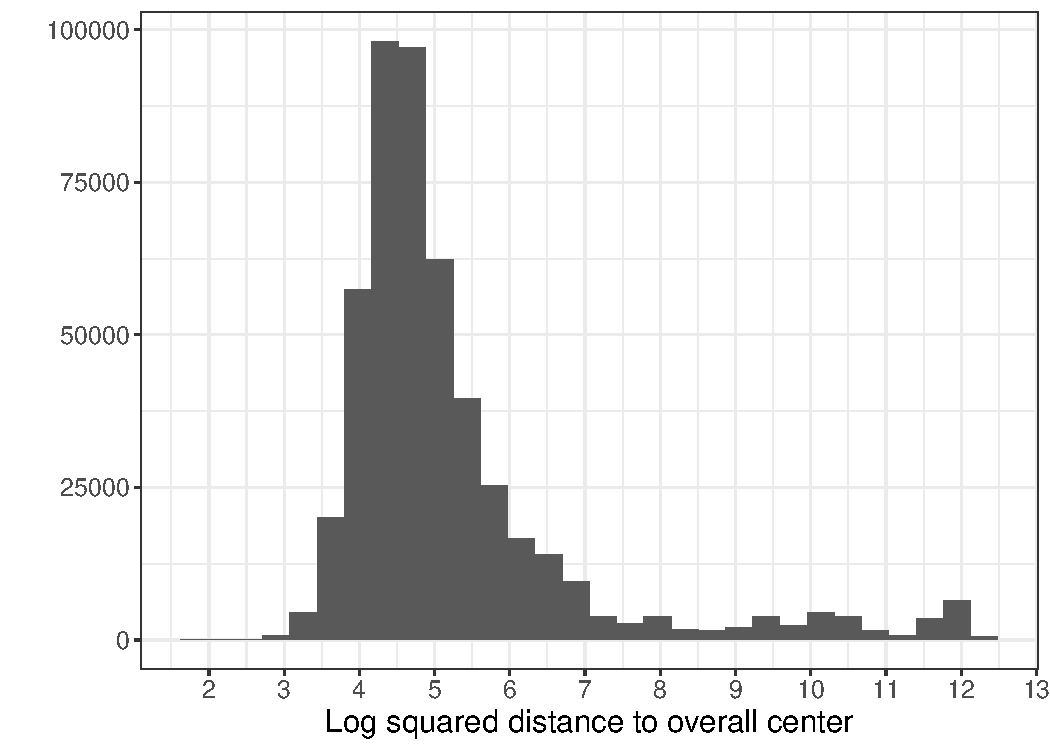
\includegraphics[width=0.8\textwidth]{hist-dist-overall-center}}
	\caption{Histogram of (log) squared distances from the UK Biobank PC scores to the geometric median of the all UKBB individuals. Here we use a threshold at 7, based on visual inspection. \label{fig:hist3}}
\end{figure}

\FloatBarrier

%%%%%%%%%%%%%%%%%%%%%%%%%%%%%%%%%%%%%%%%%%%%%%%%%%%%%%%%%%%%%%%%%%%%%%%%%%%%%%%%




\end{document}
